\documentclass[milestone1.tex]{subfiles} 
\begin{document}

%% ----------------------------------------------
% Section Experiments
%% ----------------------------------------------
\section{Experiments}




\subsection{Test Protocol}

The whole test protocol can be found on the Testmasters\footnote{https://testmaster-asl-eth.renuo.ch and https://testmaster2-asl-eth.renuo.ch}. One will find a complete list of experiments which were conducted on the Amazon cloud. Additionally, a short summary of the test protocol can be found in the directory \textit{ethz-asl-mlmq/doc/test\_protocol}.

\subsection{Testload}
To generate test load for the messaging system a mixture of different types of clients have been chosen. This section describes these clients and their behaviour.

\subsubsection{OneWayClient}
As stated in the project description each OneWayClient sends an initial message to an arbitrary other one. Having it's initial message sent they periodically check their personal queue for incoming messages. If there is one the message is dequeued and forwarded to a random receipient.

Sent messages contain a simple counter which is increased each time a message is relayed.

\subsubsection{PairedClient}
PairedClient's always come in pairs. They keep on sending requests and responses to each other. At start it is determined which client is the requesting client and which is the responding client.

\subsubsection{PublicQueueProducer}
This kind of client writes the same message again and again to a public queue.

\subsubsection{PublicQueueConsumer}
This kind of client tries to read messages at a constant rate from a public queue.


\subsection{Microbenchmarks}

The goal of the microbenchmarks is to understand single components and units.

\subsubsection{Plots}

This section starts with some plots from the microbenchmarks.

\begin{figure}[H]
	\begin{center}
    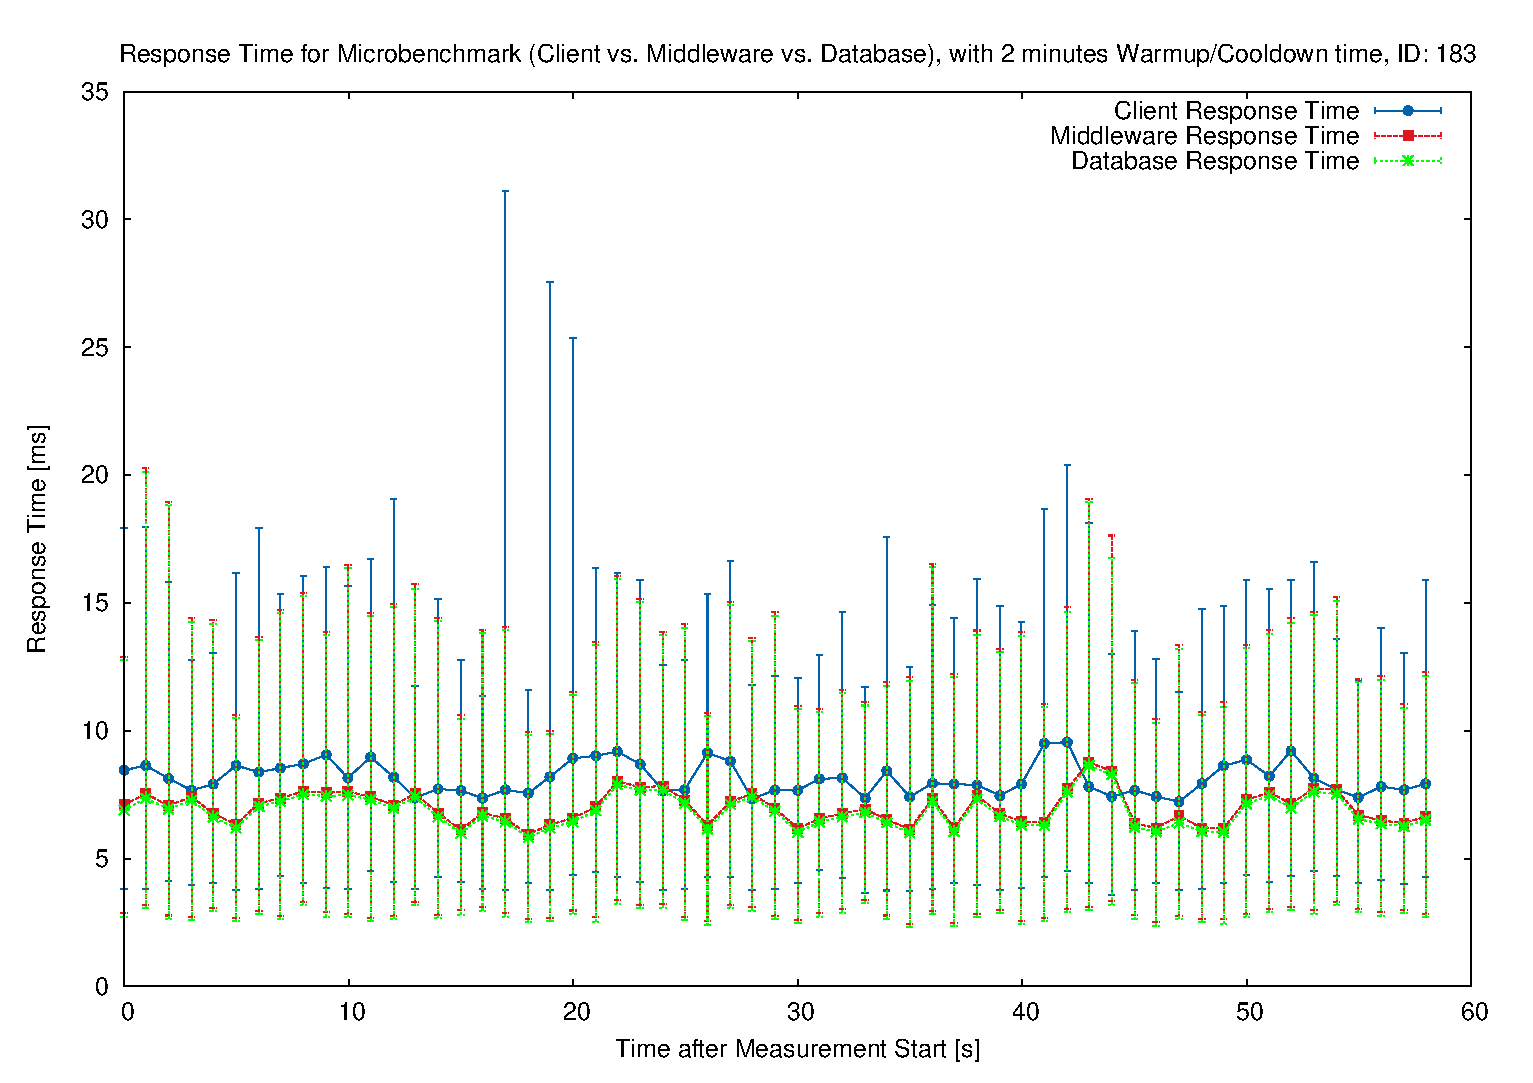
\includegraphics[scale=0.55]{../exported_plots/microbenchmarks/response_time.eps}
  \end{center}
  \caption{Response time of microbenchmark. The error bars are the 2.5\% and 97.5\% percentiles.}
  \label{fig:mictobenchmarksrt}
\end{figure}

\begin{figure}[H]
	\begin{center}
    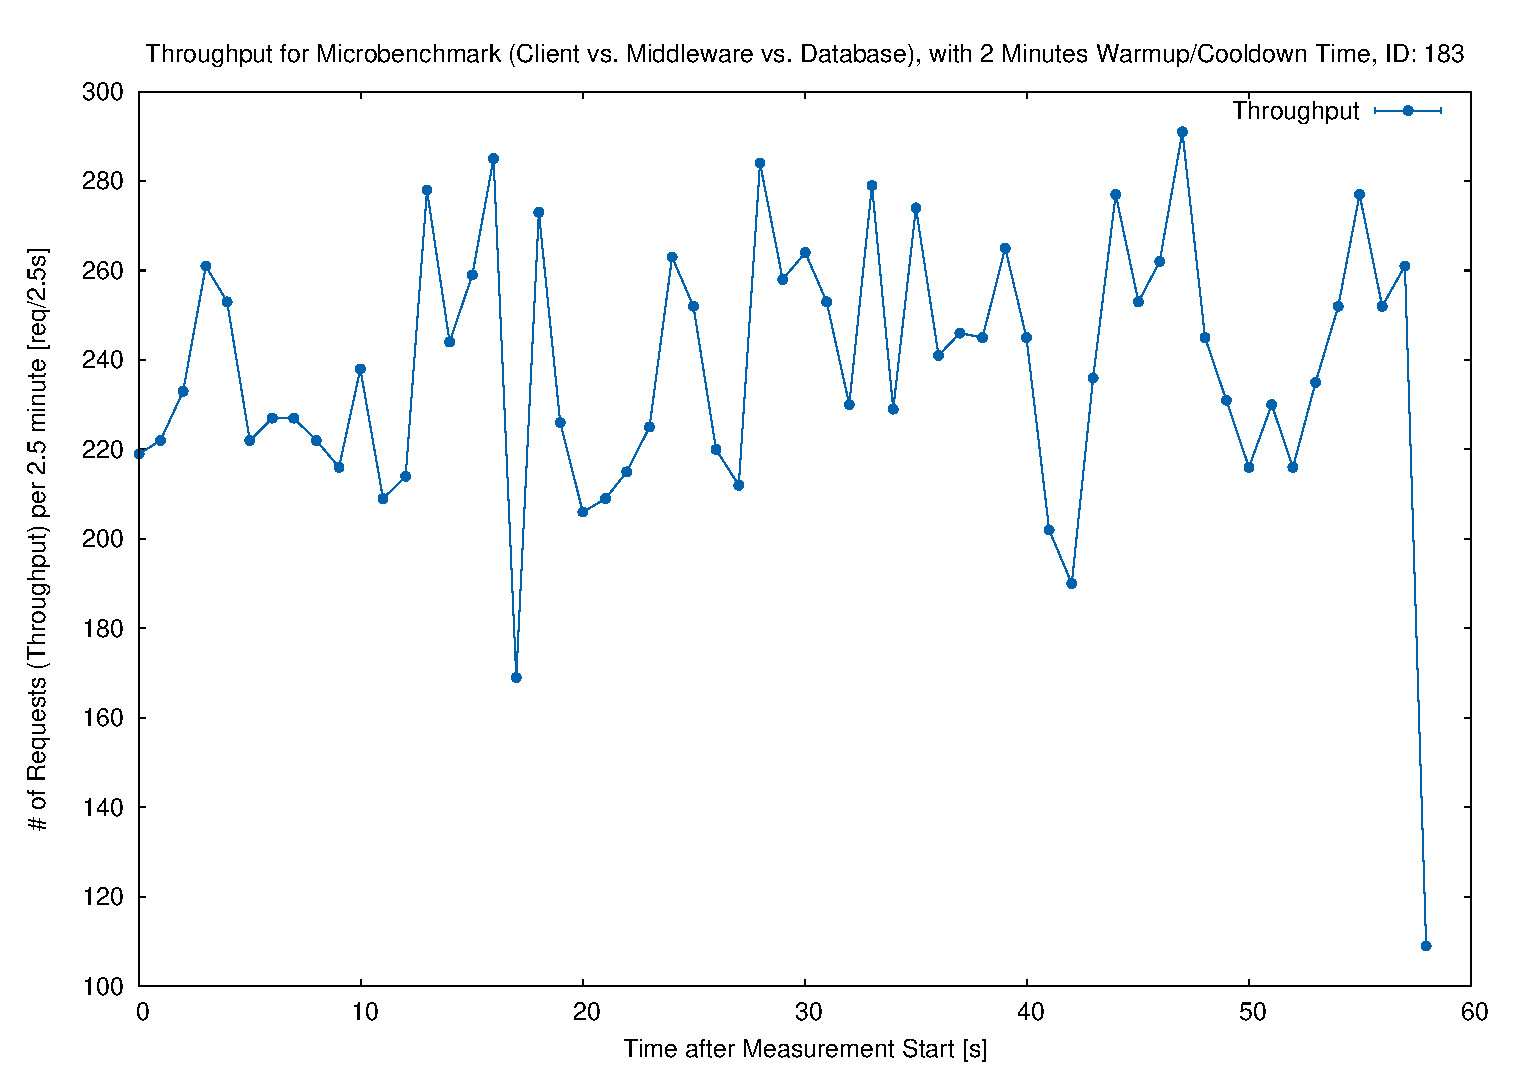
\includegraphics[scale=0.55]{../exported_plots/microbenchmarks/througput.eps}
  \end{center}
  \caption{Throughput of microbenchmark in 1000 requests.}
  \label{fig:mictobenchmarkstp}
\end{figure}


\subsubsection{Send Message and Receive Message}

The time to send a message has been measured:\\

\begin{tabular}{|l|l|r|r|r|}
\hline 
Test Run ID & Component & Median [$\mu$s] & Mean [$\mu$s] & StdDev [$\mu$s] \\ \hline
183 & Client & 6832 & 7365.251888 & 4187.470317 \\ \hline
183 & Middleware & 5467 & 5694.925436 & 2628.921725 \\ \hline
183 & Database & 5424 & 5652.727388 & 2576.826615 \\ \hline
\end{tabular}
\\\\

\noindent The time to receive a message has been measured:\\

\begin{tabular}{|l|l|r|r|r|}
\hline 
Test Run ID & Component & \textbf{Median [$\mu$s]} & Mean [$\mu$s] & StdDev [$\mu$s] \\ \hline
183 & Client & 8954 & 9796.484939 & 4927.697663 \\ \hline
183 & Middleware & 7617 & 8073.361544 & 3467.291457 \\ \hline
183 & Database & 7575 & 8029.920168 & 3461.8049 \\ \hline
\end{tabular}
\\

\noindent Calculation of the expected time for send message:

\begin{tabular}{|l|l|r|r|r|}
\hline 
Component & Type & Expected Time [$\mu$s] & Expected Time [\%] \\ \hline
\begin{tabular}[x]{@{}c@{}}Client and Network \\Client-Middleware\end{tabular} & Send & 1365 & 19.9795081967213 \\ \hline
\begin{tabular}[x]{@{}c@{}}Middleware after \\deserialization\end{tabular}  & Send & 43 & 0.629391100702576 \\ \hline
\begin{tabular}[x]{@{}c@{}}Database and Network \\Middleware-Database\end{tabular} & Send & 5424 & 79.3911007025761 \\ \hline
\end{tabular}
\\

\noindent And the following results for the receive message:\\

\begin{tabular}{|l|l|r|r|r|}
\hline 
Component & Type & Expected Time [$\mu$s] & Expected Time [\%] \\ \hline
\begin{tabular}[x]{@{}c@{}}Client and Network \\Client-Middleware\end{tabular} & Receive & 1337 & 14.9318740227831 \\ \hline
\begin{tabular}[x]{@{}c@{}}Middleware after \\deserialization\end{tabular}  & Receive & 42 & 0.469064105427742 \\ \hline
\begin{tabular}[x]{@{}c@{}}Database and Network \\Middleware-Database\end{tabular} & Receive & 7575 & 84.5990618717892\\ \hline
\end{tabular}
\\

\paragraph{Interpretation} The think time of the client should be very near to 0ms - so we use the same value here as for the broker. Thus, we suspect that the difference between client and middleware is the network. We assume that the network time between the client and the middleware is the same as the middleware and the database.  We consider the median for the measurements.\\
This way, we can estimate the network as $2*(client-middleware)$, and the client as $middleware$. Also, the database should be $database-network/2$.
Thus we conclude the following final results for the send message:\\

\begin{tabular}{|l|l|r|r|r|}
\hline
Component & Type & Expected Time [$\mu$s] & Expected Time [\%] \\ \hline
Client & Send & 43 & 0.629391100702576 \\ \hline
Middleware & Send & 43 & 0.629391100702576 \\ \hline
Database & Send & 4016 & 58.7822014051522 \\ \hline
Network & Send & 2644 & 38.7002341920375 \\ \hline
\end{tabular}
\\

\noindent And the following final results for the receive message:\\

\begin{tabular}{|l|l|r|r|r|}
\hline
Component & Type & Expected Time [$\mu$s] & Expected Time [\%] \\ \hline
Client & Receive & 42 & 0.469064105427742 \\ \hline
Middleware & Receive & 42 & 0.469064105427742 \\ \hline
Database & Receive & 6196 & 69.1981237435783 \\ \hline
Network & Receive & 2590 & 28.9256198347107 \\ \hline
\end{tabular}
\\



\subsubsection{Time Caused By Code}

As described in the previous section, the time used for the code is 0.042 ms and 0.043 ms for sending and receiving respectively. In percent this is less then 1\% for sending and receiving, and thus this factor is relatively unimportant compared to the database and the network.

TODO...


\subsubsection{Network performance}

Even though the network connection throughput is specified by Amazon, only a measurement tells the truth. To confirm this, a network performance test was executed with iperf. We simulated a bi-directional data transfer between a middleware/client and the database. We get about 841Mbits/s upload to the database and 93.1Mbits/s download to the middleware/client if iperf is run in bidirectional mode (send and receive in parallel. If only one direction is used, then the throughput from middleware/client to database is 959Mbits/s and from database to middleware/client it is about 312Mbits/s. We also notice that the variance for the single values are rather big.\\

\begin{figure}[H]
\begin{center}
\begin{verbatim}
------------------------------------------------------------
Client connecting to 54.194.38.184, TCP port 5001
TCP window size:  133 KByte (default)
------------------------------------------------------------
[  3] local 172.31.6.201 port 60902 connected with 54.194.38.184 port 5001
[  5] local 172.31.6.201 port 5001 connected with 54.194.38.184 port 52555
[ ID] Interval       Transfer     Bandwidth
[  3]  0.0-10.0 sec   122 MBytes   102 Mbits/sec
[  5]  0.0-10.0 sec   970 MBytes   814 Mbits/sec
[  5] 10.0-20.0 sec  1007 MBytes   844 Mbits/sec
[  3] 10.0-20.0 sec   135 MBytes   113 Mbits/sec
[  5] 20.0-30.0 sec  1.00 GBytes   861 Mbits/sec
[  3] 20.0-30.0 sec   121 MBytes   102 Mbits/sec
[  5] 30.0-40.0 sec   978 MBytes   820 Mbits/sec
[  3] 30.0-40.0 sec   111 MBytes  93.0 Mbits/sec
[  5] 40.0-50.0 sec  1009 MBytes   846 Mbits/sec
[  3] 40.0-50.0 sec  88.0 MBytes  73.8 Mbits/sec
[  5] 50.0-60.0 sec  1.00 GBytes   862 Mbits/sec
[  3] 50.0-60.0 sec  89.1 MBytes  74.8 Mbits/sec
[  3]  0.0-60.1 sec   666 MBytes  93.1 Mbits/sec
[  5]  0.0-60.0 sec  5.88 GBytes   841 Mbits/sec
\end{verbatim}
\end{center}
\caption{Bidirectional Test}
\label{fig:iperfclient}
\end{figure}

\begin{figure}[H]
\begin{center}
\begin{verbatim}
------------------------------------------------------------
Client connecting to 54.194.38.184, TCP port 5001
TCP window size: 22.9 KByte (default)
------------------------------------------------------------
[  3] local 172.31.6.201 port 60905 connected with 54.194.38.184 port 5001
[ ID] Interval       Transfer     Bandwidth
[  3]  0.0-10.0 sec   430 MBytes   361 Mbits/sec
[  3] 10.0-20.0 sec   342 MBytes   287 Mbits/sec
[  3] 20.0-30.0 sec   347 MBytes   291 Mbits/sec
[  3] 30.0-40.0 sec   426 MBytes   357 Mbits/sec
[  3] 40.0-50.0 sec   342 MBytes   287 Mbits/sec
[  3] 50.0-60.0 sec   342 MBytes   287 Mbits/sec
[  3]  0.0-60.0 sec  2.18 GBytes   312 Mbits/sec
\end{verbatim}
\end{center}
\caption{Unidirectional test, database to middleware / client}
\label{fig:iperfserver}
\end{figure}


\begin{figure}[H]
\begin{center}
\begin{verbatim}
------------------------------------------------------------
Client connecting to 54.194.42.48, TCP port 5001
TCP window size: 22.9 KByte (default)
------------------------------------------------------------
[  3] local 172.31.8.61 port 52558 connected with 54.194.42.48 port 5001
[ ID] Interval       Transfer     Bandwidth
[  3]  0.0-10.0 sec  1.13 GBytes   974 Mbits/sec
[  3] 10.0-20.0 sec  1.11 GBytes   956 Mbits/sec
[  3] 20.0-30.0 sec  1.11 GBytes   957 Mbits/sec
[  3] 30.0-40.0 sec  1.11 GBytes   957 Mbits/sec
[  3] 40.0-50.0 sec  1.11 GBytes   956 Mbits/sec
[  3] 50.0-60.0 sec  1.11 GBytes   956 Mbits/sec
[  3]  0.0-60.0 sec  6.70 GBytes   959 Mbits/sec

\end{verbatim}
\end{center}
\caption{Unidirectional test, middleware/client to database}
\label{fig:iperfserver2}
\end{figure}

Sending one message uses about 20 Bytes without payload, because we use custom serialization \ref{sub:des-msg-ser} \nameref{sub:des-msg-ser}. Thus, our message size will be between 20 Bytes and 2020 Bytes. With a network connection that supports 100Mbit/s we can send 625'000 (without payload) up to 6188 (with payload) per second. In this project we focus on messages without / only little payload, and thus the network bandwidth is not a bottleneck for the throughput for the tests.


\subsubsection{Component Limits}

In the microbenchmarks, the limit for the amount of messages a single client was determined:\\

\begin{tabular}{|l|l|r|r|r|}
\hline
Duration [s] & Requests sent \\ \hline
100 & 23465 \\ \hline
\textbf{1} & \textbf{234.65} \\ \hline
\end{tabular}
\\





\subsubsection{Testmaster}

To run the tests, the Testmaster is used to compile the Java code, generate the config files, deploy it to the Amazon AWS machines and start the tests. When the test finishes, it then copies all log files after all Java JVM's have stopped. This whole process takes 8-9 minutes when the Java instances stop immediately.




\subsection{2 Hour Test}


% for each experiment
%- why are we doing this experiment
%- hypothesis
%- experiment setup (parameters)
%- plots of the result
%- describe the plot
%- explain the plot/experiment

To verify that the system runs stable over a long period of time an experiment is performed which puts a constant load onto the system for 2 hours.\\

During the project, the system evolved and thus some test runs were invalidated in this process. Here, the final two 2h test runs are presented. The other 2h test runs can be found and analysed on the Testmaster\footnote{https://testmaster-asl-eth.renuo.ch/}.\\

\subsubsection{Experiment setup}
The experiment is performed on the Amazon cloud with constant load. For the setup configuration, the project specifications were used specifications (80 clients).\\

\begin{tabular}{|l|l|}
\hline 
Amazon instance type and availability zone & Value \\
\hline 
database & m1.medium, eu-west-1a \\ 
middlewares & m1.small, eu-west-1a \\ 
clients & m1.small, eu-west-1a \\ 
\hline 
\end{tabular}


\paragraph{Middleware} In total 6 middleware components are running On 2 Amazon instances.

\paragraph{Clients} The following mix of clients are used for the 2 hour test.

\begin{tabular}{|l|c|c|}
\hline 
\textbf{Client type mix } & \# \\ 
\hline 
OneWayClient & 1x30 (machines x jvms)  \\ 
\hline 
PairedClient & 1x16 (machines x jvms) \\ 
\hline 
PublicQueueConsumer & 1x10 (machines x jvms) \\ 
\hline 
PublicQueueProducer & 1x5 (machines x jvms) \\ 
\hline 
\end{tabular} 


\subsubsection{Hypothesis}
Since the system will not be saturated we expect no changes over time concerning response time and throughput. The mixture of clients generating load is chosen such that there is a constant number of messages in the system. Increased SQL query execution time should not be observable.

\subsubsection{Results}
There were multiple 2h tests performed. The final two 2h tests are the ones with id 174 \footnote{https://testmaster-asl-eth.renuo.ch/test\_runs/174} and 176 \footnote{https://testmaster-asl-eth.renuo.ch/test\_runs/176}. Both run stable and generated the following plots:


% ------------------------------------------------
\begin{figure}[H]
  \begin{center}
    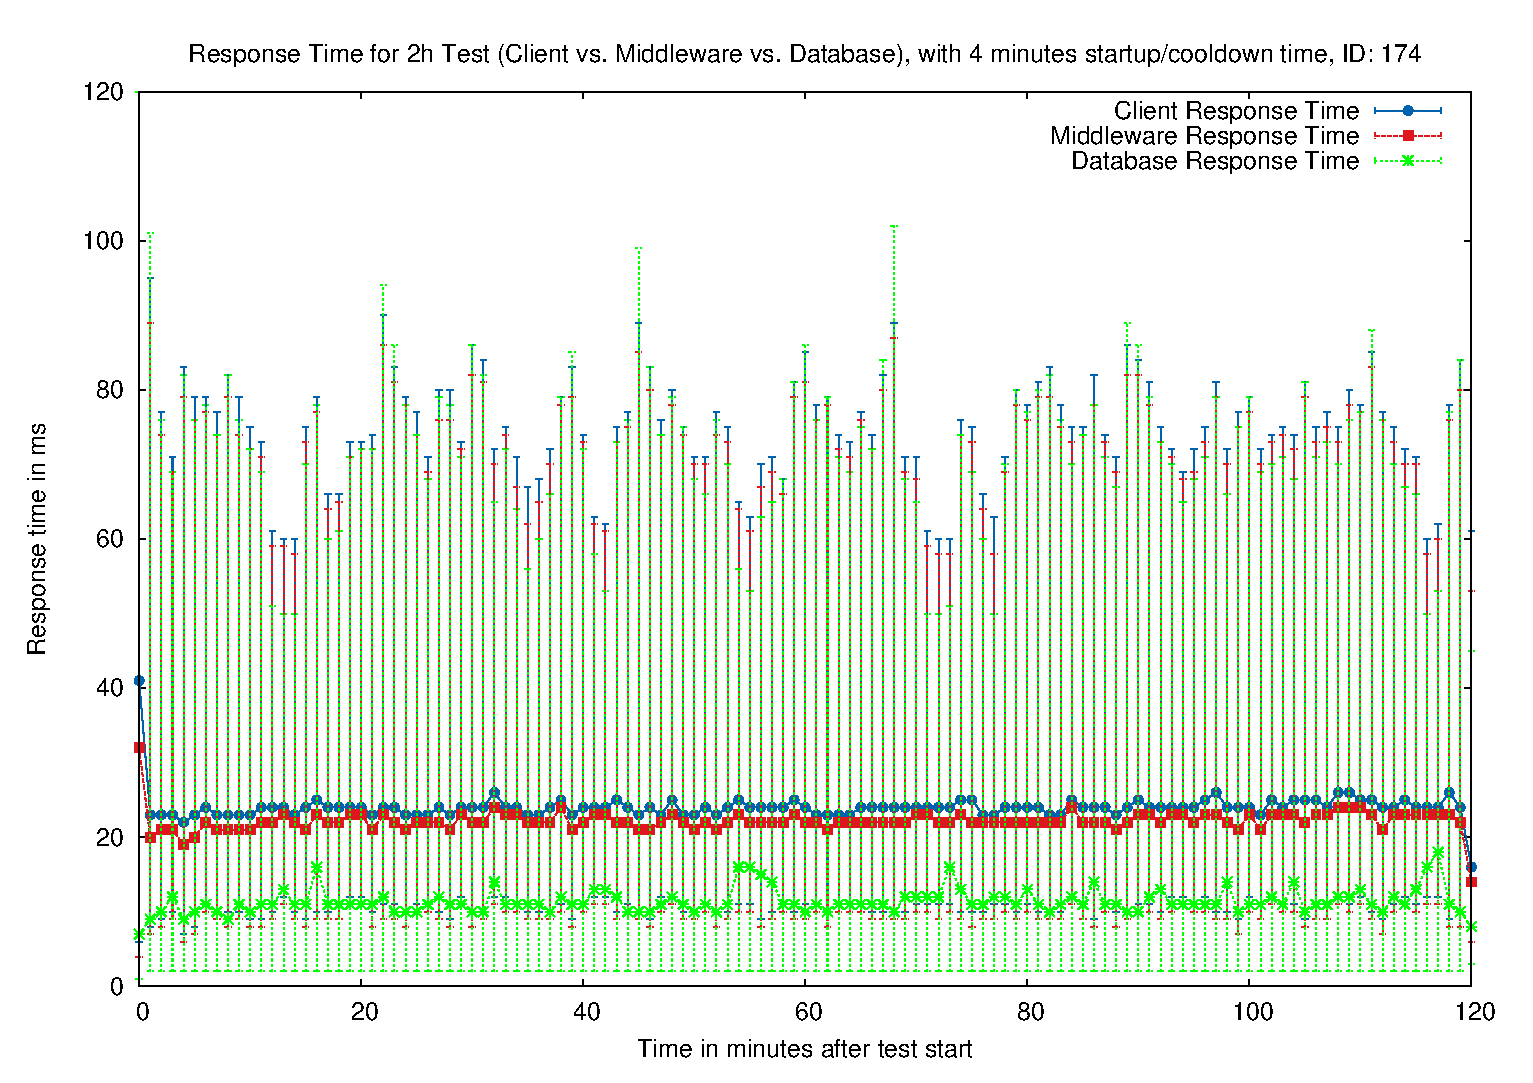
\includegraphics[scale=0.6]{../exported_plots/2h/174_rt-final.eps}
  \end{center}
  \caption{Response time of 2h Test. The error bars are the 2.5\% and 97\% percentiles}
  \label{fig:2htest-plot-rt}
\end{figure}


% ------------------------------------------------
\begin{figure}[H]
  \begin{center}
    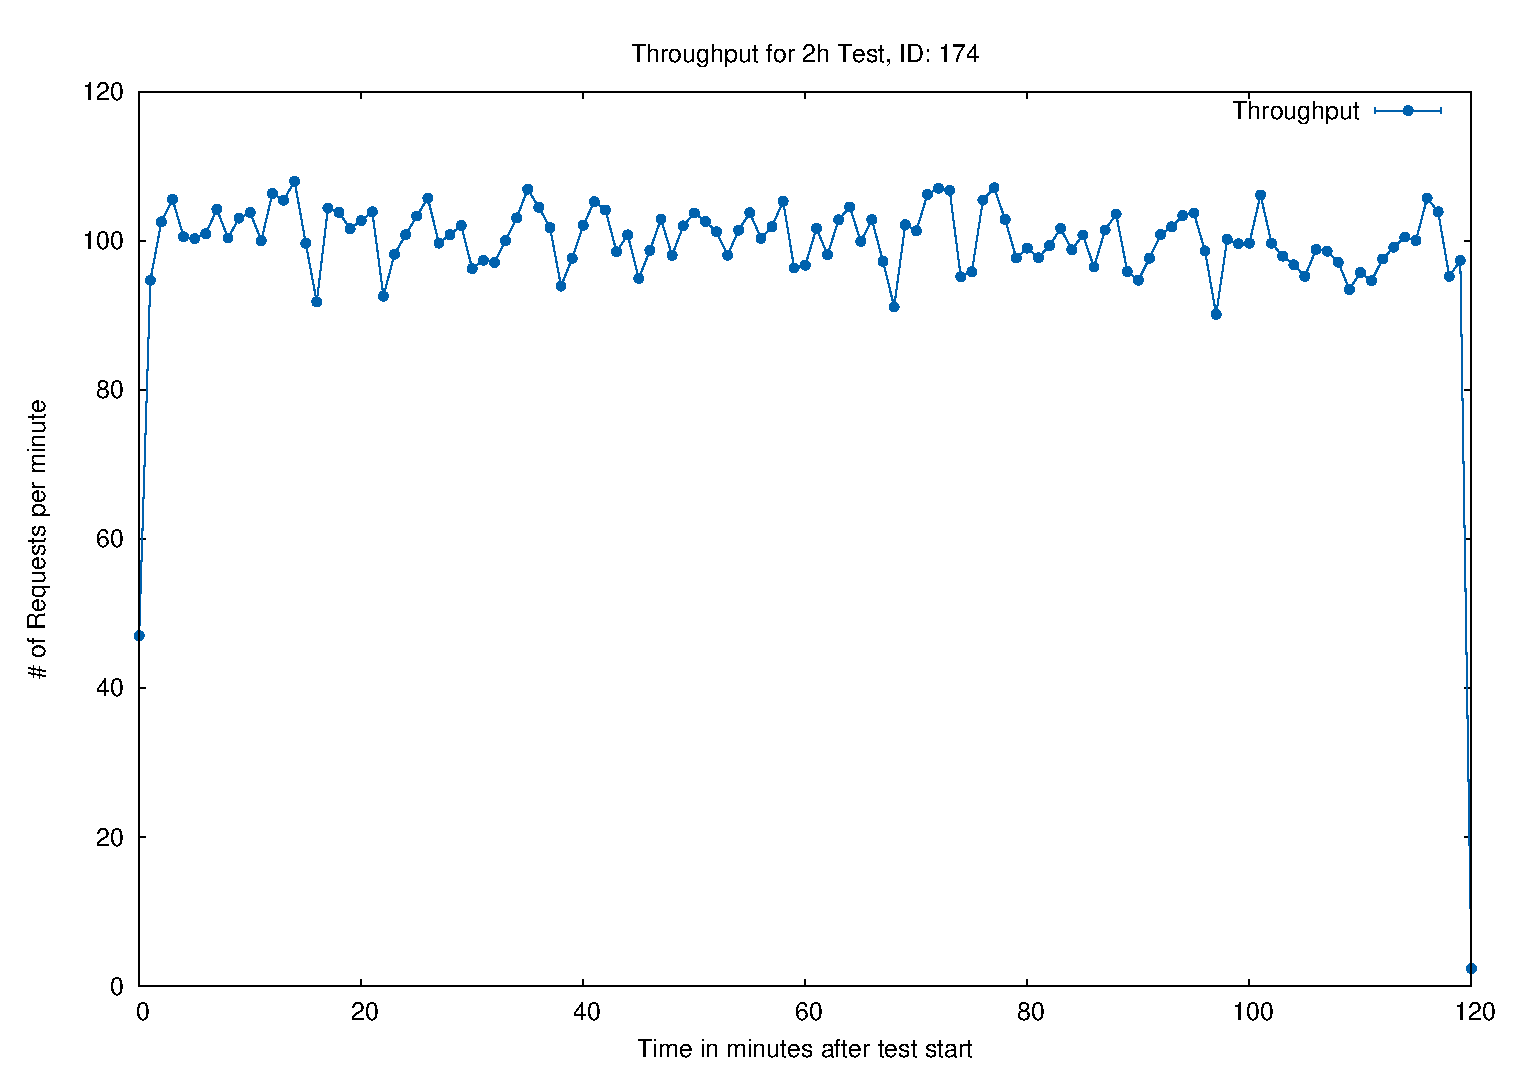
\includegraphics[scale=0.6]{../exported_plots/2h/174_tp-final.eps}
  \end{center}
  \caption{Throughput of 2h test in 1000 requests.}
  \label{fig:2htest-plot-tp}
\end{figure}




\subsubsection{Interpretation}
The final test runs (174 and 176) run as expected in the hypothesis.

%% -------------------------------------------
%% 2^k Experiment
%% -------------------------------------------
\subsection{$2^k$ Experiment}
In order to determine the influence of a number of primary factors on to the system it was decided to do a $2^k$ analysis on several factors described in the following section.

For each feature level an experiment of 30 minutes is performed where clients perform 100 actions (send and receive message) per second.

\subsubsection{Factors and Levels}

\paragraph{Number of Clients}
The number of simultaneously connected clients is varied between 8 and 30. There is a mix of different clients which produce slightly different types of load.

\begin{tabular}{|l|c|c|}
\hline 
\textbf{Client type mix } & \# & \# \\ 
\hline 
OneWayClient & 16 & 8  \\ 
\hline 
PairedClient & 8 & 4 \\ 
\hline 
PublicQueueConsumer & 4 & 2 \\ 
\hline 
PublicQueueProducer & 2 & 1 \\ 
\hline 
\textbf{Total}  & \textbf{30} & \textbf{15} \\
\hline 
\end{tabular} 

\paragraph{Number of brokers}

The number of middleware components is varied between 4 and 8. For both levels the number of Amazon instances used is 2.

\paragraph{Number of workers}

The number of worker threads a single middleware instance has is varied between 4 and 8

\paragraph{Number of Database Connections}

The number of concurrent database connection a single middleware instance has is varied between 4 and 8


\subsubsection{Hypothesis}

The response time should not be majorly affected by these chosen parameters. Since the system is not under much load only small changes concerning the response time should be observable.

However the number of requests processes should vary. The main feature which obviously affects number of requests is the number of connected clients sending messages. Other minor variations will reveal bottle necks in the system.

\subsubsection{Measurement Results}
The following table shows median time taken and number of requests processed for all different feature levels.\\

\begin{figure}[H]
	\begin{center}
	
\begin{tabular}{cccccccc}
\rot{Clients C} & 
\rot{Brokers B} & 
\rot{Workers W} & 
\rot{Connections D} & 
\rot{TestRun Id} & 
\rot{Median Processing time [ms] PT} & 
\rot{\# of Processed Requests RC} \\
\hline 
15 & 4 & 4 & 4 & 2003 & \numprint{6.80} & \numprint{1996478} \\ 
\hline 
15 & 4 & 4 & 8 & 173 & \numprint{7.46} & \numprint{1806665} \\ 
\hline 
15 & 4 & 8 & 4 & 2007 & \numprint{6.87} & \numprint{2062704} \\ 
\hline 
15 & 4 & 8 & 8 & 2008 & \numprint{7.21}  & \numprint{2060655} \\ 
\hline 
15 & 8 & 4 & 4 & 2009 & \numprint{5.11} & \numprint{1385552} \\ 
\hline 
15 & 8 & 4 & 8 & 2004 & \numprint{7.55} & \numprint{1910840} \\ 
\hline 
15 & 8 & 8 & 4 & 2005 & \numprint{5.90} & \numprint{1975889} \\ 
\hline 
15 & 8 & 8 & 8 & 2006 & \numprint{7.60} & \numprint{1920835} \\ 
\hline 
30 & 4 & 4 & 4 & 159 & \numprint{14.08} & \numprint{2488948} \\ 
\hline 
30 & 4 & 4 & 8 & 160 & \numprint{12.80} & \numprint{2451248} \\ 
\hline 
30 & 4 & 8 & 4 & 161 & \numprint{13.42} & \numprint{2428769} \\ 
\hline 
30 & 4 & 8 & 8 & 162 & \numprint{13.97} & \numprint{2511260}  \\ 
\hline 
30 & 8 & 4 & 4 & 163 & \numprint{12.43} & \numprint{2329883} \\ 
\hline 
30 & 8 & 4 & 8 & 164 & \numprint{14.85} & \numprint{2110459} \\ 
\hline 
30 & 8 & 8 & 4 & 165 & \numprint{12.88} & \numprint{2266237} \\ 
\hline 
30 & 8 & 8 & 8 & 166 & \numprint{15.05} & \numprint{2166303}  \\ 
\hline 

\end{tabular} 
\end{center}
\caption{$2^4$ factorial test measurements}
\label{fig:2kfactorialmeasurement}
\end{figure}

\paragraph{Signs}

For the $2^k$ test the following signs are assigned to feature leavels:\\


\begin{figure}[H]
	\begin{center}
\begin{tabular}{|l|c|c|}
\hline 
\textbf{Feature} & \textbf{+1 Level} & \textbf{-1 Level} \\ 
\hline 
Number of Clients \textbf{C} & 30 & 15 \\ 
\hline 
Number of Brokers \textbf{B} & 8 & 4 \\ 
\hline 
Number of Workers \textbf{W} & 8 & 4 \\ 
\hline 
Number of Database Connections \textbf{D} & 8 & 4 \\ 
\hline 
\end{tabular} 
\end{center}
\caption{Feature Level Signs}
\end{figure}

This leads to the following sign table.


\begin{figure}[H]
	\begin{center}
\begin{tabular}{ccccccccccccccccc}
\hline 
 & I &	c&	b&	w&	d&	cb&	cw&	cd&	bw&	bd&	wd&	bwd&	cwd&	cbd&	cbw&	cbwd \\
\hline 
&1&	-1&	-1&	-1&	-1&	1&	1&	1&	1&	1&	1&	-1&	-1&	-1&	-1&	1 \\
&1&	-1&	-1&	-1&	1&	1&	1&	-1&	1&	-1&	-1&	1&	1&	1&	-1&	-1 \\
&1&	-1&	-1&	1&	-1&	1&	-1&	1&	-1&	1&	-1&	1&	1&	-1&	1&	-1 \\
&1&	-1&	-1&	1&	1&	1&	-1&	-1&	-1&	-1&	1&	-1&	-1&	1&	1&	1 \\
&1&	-1&	1&	-1&	-1&	-1&	1&	1&	-1&	-1&	1&	1&	-1&	1&	1&	-1 \\
&1&	-1&	1&	-1&	1&	-1&	1&	-1&	-1&	1&	-1&	-1&	1&	-1&	1&	1 \\
&1&	-1&	1&	1&	-1&	-1&	-1&	1&	1&	-1&	-1&	-1&	1&	1&	-1&	1 \\
&1&	-1&	1&	1&	1&	-1&	-1&	-1&	1&	1&	1&	1&	-1&	-1&	-1&	-1 \\
&1&	1&	-1&	-1&	-1&	-1&	-1&	-1&	1&	1&	1&	-1&	1&	1&	1&	-1 \\
&1&	1&	-1&	-1&	1&	-1&	-1&	1&	1&	-1&	-1&	1&	-1&	-1&	1&	1 \\
&1&	1&	-1&	1&	-1&	-1&	1&	-1&	-1&	1&	-1&	1&	-1&	1&	-1&	1 \\
&1&	1&	-1&	1&	1&	-1&	1&	1&	-1&	-1&	1&	-1&	1&	-1&	-1&	-1 \\
&1&	1&	1&	-1&	-1&	1&	-1&	-1&	-1&	-1&	1&	1&	1&	-1&	-1&	1 \\
&1&	1&	1&	-1&	1&	1&	-1&	1&	-1&	1&	-1&	-1&	-1&	1&	-1&	-1 \\
&1&	1&	1&	1&	-1&	1&	1&	-1&	1&	-1&	-1&	-1&	-1&	-1&	1&	-1 \\
&1&	1&	1&	1&	1&	1&	1&	1&	1&	1&	1&	1&	1&	1&	1&	1 \\

\hline 

\rot[90]{\textbf{Weights PT~}} & 
\rot[90]{\textbf{10.24}} &	
\rot[90]{\textbf{3.43}} &	
\rot[90]{-0.07} &	
\rot[90]{0.11} &	
\rot[90]{\textbf{0.56}} &	
\rot[90]{0.19} &	
\rot[90]{0.03} &	
\rot[90]{-0.08} &	
\rot[90]{0.07} &	
\rot[90]{\textbf{0.52}} &	
\rot[90]{0.03} &	
\rot[90]{-0.15} &	
\rot[90]{0.16} &	
\rot[90]{0.13} &	
\rot[90]{-0.05} &	
\rot[90]{-0.10} \\
\hline 

\rot[90]{\textbf{Weights RC~}} & 
\rot[90]{\numprint{2117045}} &      
\rot[90]{\numprint{227093}} & 
\rot[90]{\numprint{-108795}} & 
\rot[90]{\numprint{57036}} & 
\rot[90]{\numprint{237}} & 
\rot[90]{\numprint{-17122}} & 
\rot[90]{\numprint{-58032}} & 
\rot[90]{\numprint{-34558}} & 
\rot[90]{\numprint{17030}} & 
\rot[90]{\numprint{18621}} & 
\rot[90]{\numprint{-9556}} & 
\rot[90]{\numprint{-48050}} & 
\rot[90]{\numprint{39516}} & 
\rot[90]{\numprint{-64140}} & 
\rot[90]{\numprint{-17984}} & 
\rot[90]{\numprint{47962}} \\


\end{tabular}
\end{center}
\caption{$2^4$ factorial test result}
\label{fig:2kfactorialresults}
\end{figure}

\subsubsection{Interpretation}
It was chosen to ignore the calculated weights for processed request counts RC because big values are more difficult to read and because both observed values correlate quite well (what is shown in \ref{fig:2kmeasuredresults}.


%TODO - graphik ersetzen (Luke excel)
\begin{figure}[H]
	\begin{center}
    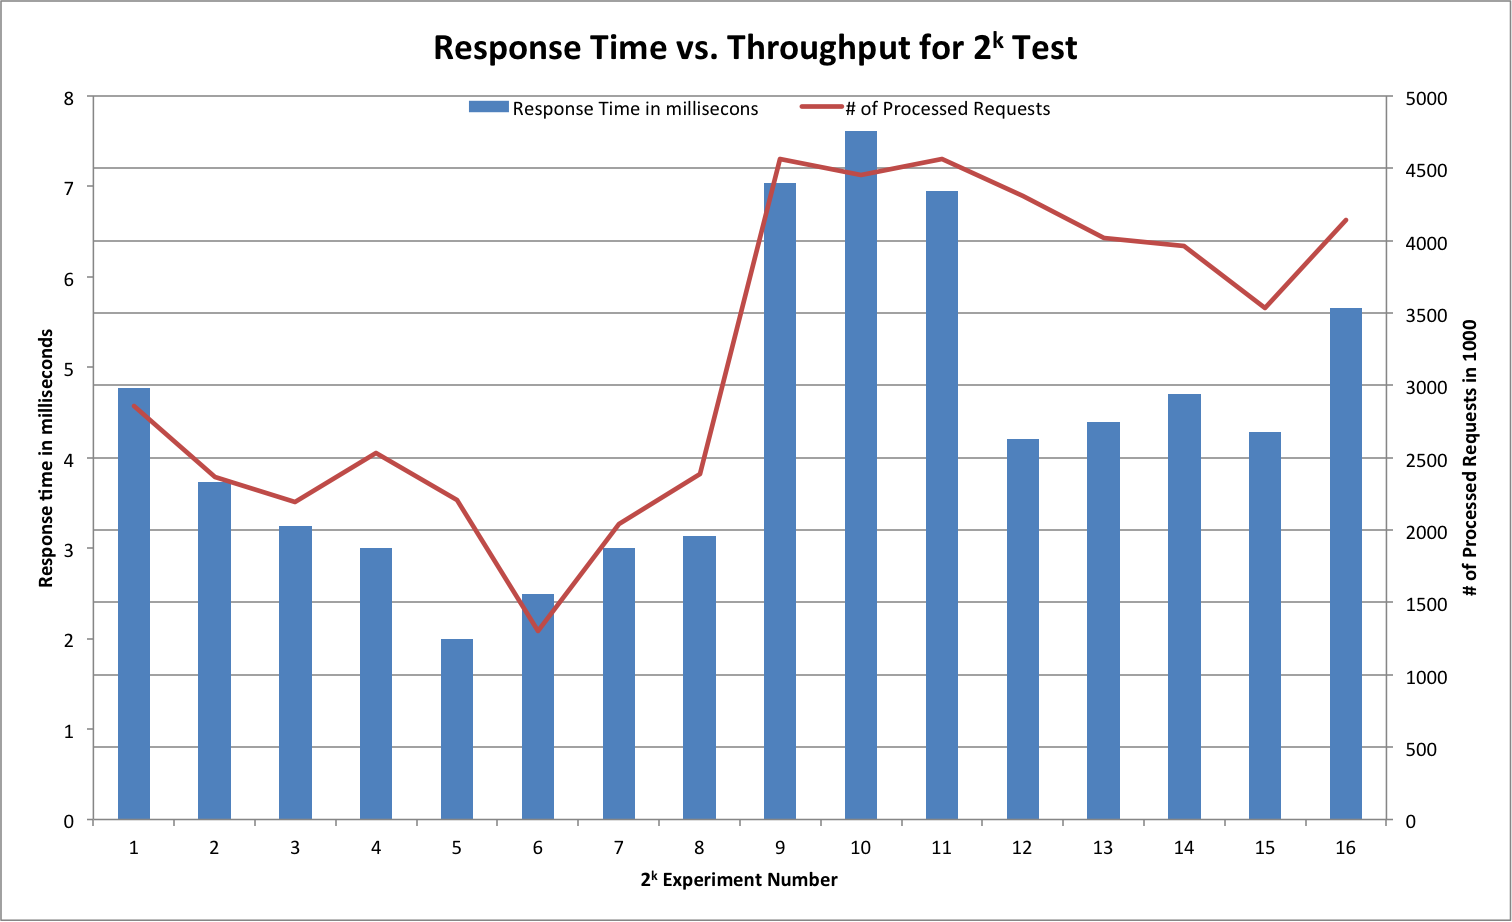
\includegraphics[scale=0.55]{../drawings/2k-factorial-plot.png}
  \end{center}
  \caption{$2^4$ factorial measured results}
  \label{fig:2kmeasuredresults}
\end{figure}



Mean performance concerning response time has a value of $10.24$. The effect of varying number of clients from 15 to 30 has a weight of $3.43$. This means when increasing the number of clients (and number of requests) the response time also increases. The other values are relatively low. Number of database connections $d$ and number of brokers $b$ in combination with number of database connections  are the next values worth to have a look at. This means that the number of database connections has the most significant impact on response time. By varying number of brokers the total number of database connections also change.

Overall the most significant factor which affects performance the most (beside the load applied by clients) is the number of database connections. This indicates that the database is a bottle neck.

%% -------------------------------------------


\subsection{Database Load Test}
To check the limits of the system a load test was performed where we start with a fixed number of middle ware instances and gradually increase the number of connected clients.

\paragraph{Middle Ware}
In total 16 middle ware instances are evenly spread across 4 Amazon instances. Each middle ware has 20 WorkerThreads and 15 concurrent database connections.

\paragraph{Clients}
Every 2 minute 20 OneWayClients try to connect. Each client tries to send and receive messages as fast as possible. In total 450 clients are spread across 15 Amazon instances (30 clients per instance).

RequestTimeout is set to 1 second. A request is considered to be successful if processed within that bound. 

\subsubsection{Hypothesis}

By increasing the load on the system both response time and throughput should increase to a certain degree. By increasing the load more the system should become unstable and start trashing.

\subsubsection{Results}

% ---------------------------------------
\begin{figure}[H]
        \begin{center}
    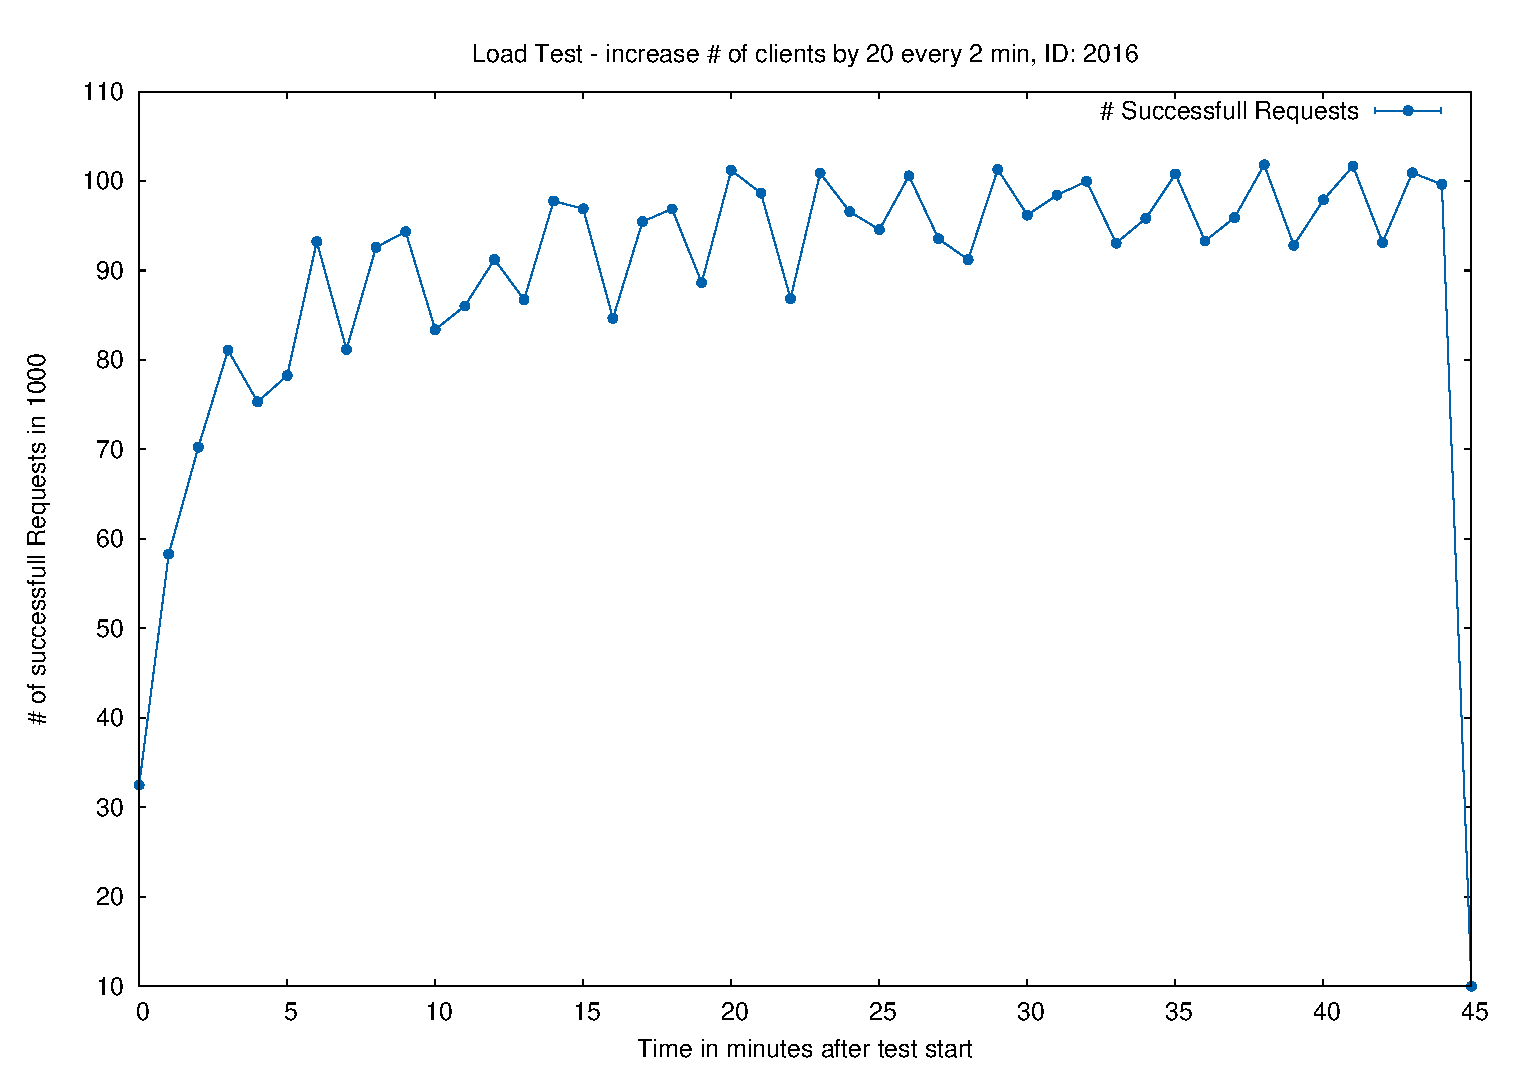
\includegraphics[scale=0.5]{../exported_plots/LoadTest/2016_NrOfGoodRequests.eps}
  \end{center}
  \caption{Throughput of load test in 1000 requests.}
  \label{fig:LoadTestThrougput}
\end{figure}
% ---------------------------------------

% ---------------------------------------
\begin{figure}[H]
        \begin{center}
    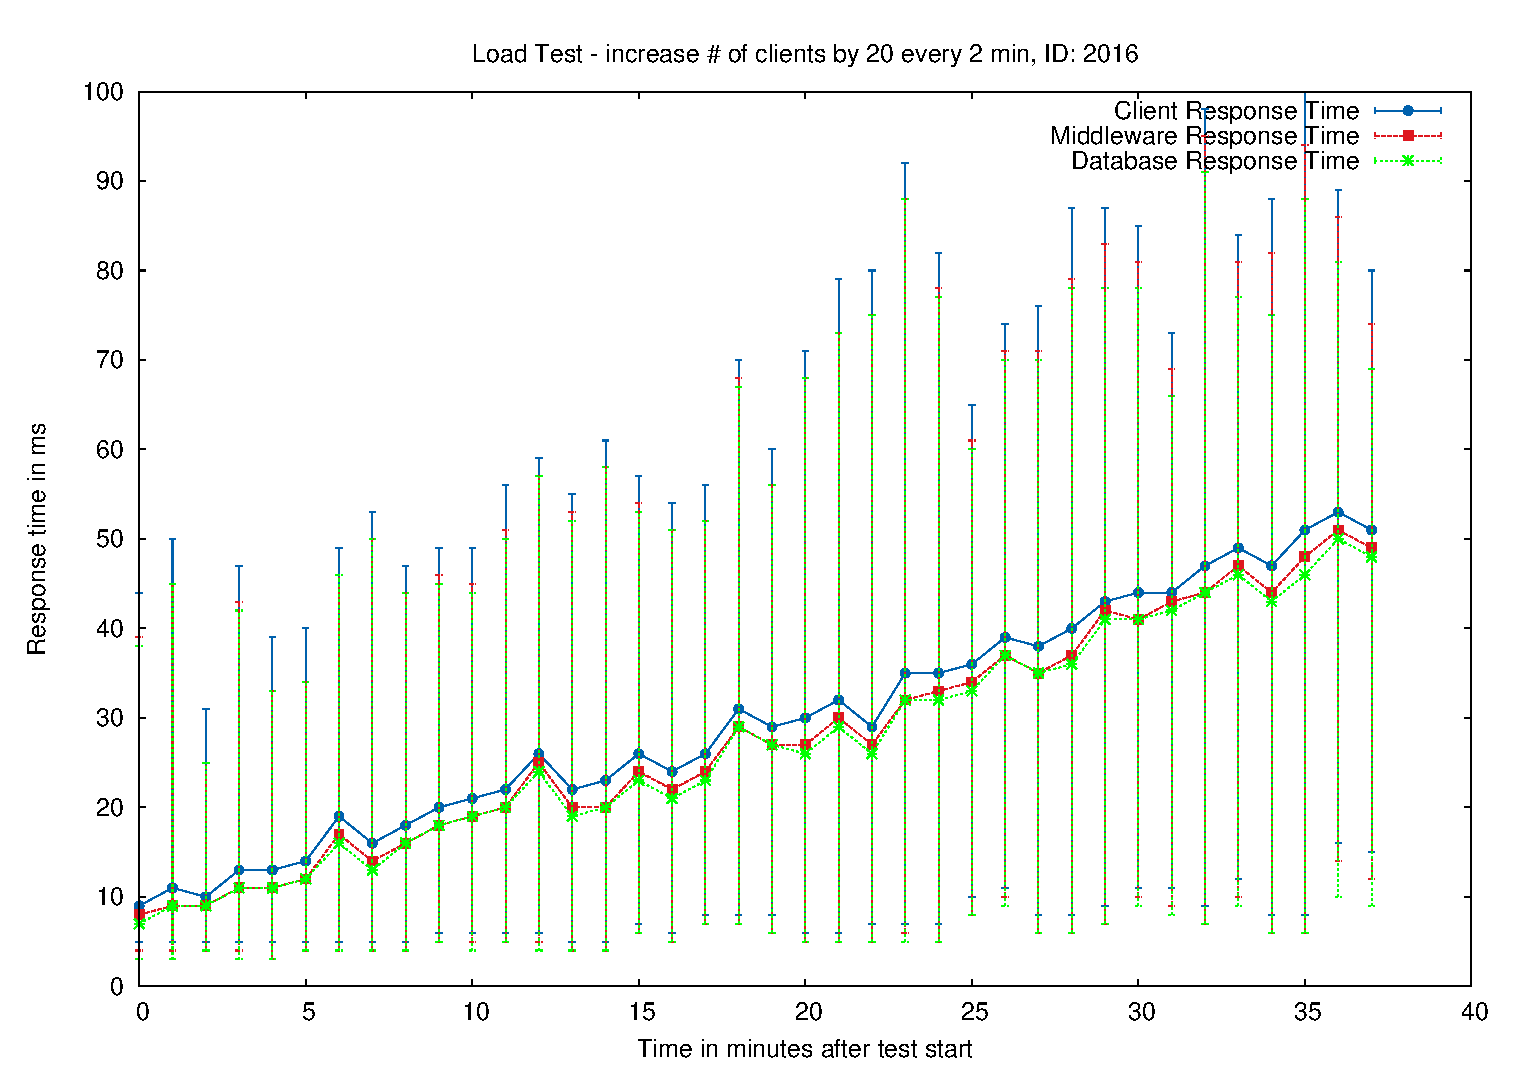
\includegraphics[scale=0.5]{../exported_plots/LoadTest/2016_ResponseTime.eps}
  \end{center}
  \caption{Response time of Load Test. The error bars are the 2.5\% and 97.5\% percentiles.}
  \label{fig:LoadTestResponseTime}
\end{figure}
% ---------------------------------------

\subsubsection{Interpretation}

As expected the response time increases as the load on the system gets higher. Also worth mentioning is that the lines in Figure \ref{fig:LoadTestResponseTime} remain parallel. This means that the all component except the database remain stable concerning response time. The database needs more and more time to process queries while load is increased.

The number of successfully processed requests reaches its peak between 5 and 10 minutes (approximate with 80 clients). The system is then saturated.

This result is quite disappointing since it does not support our hypothesis. That type of experiment was repeated several times while increasing the number of total clients and still the system seems not to be saturated. It was decided to not repeat the experiment with even more clients (because our Amazon voucher was used up).


\subsection{Middleware Load Test}
To check the limits of a single middleware instance a load test is performed with a single instance.


\subsubsection{Hypothesis}



\subsubsection{Results}

% ------------------------------
\begin{figure}[H]
        \begin{center}
    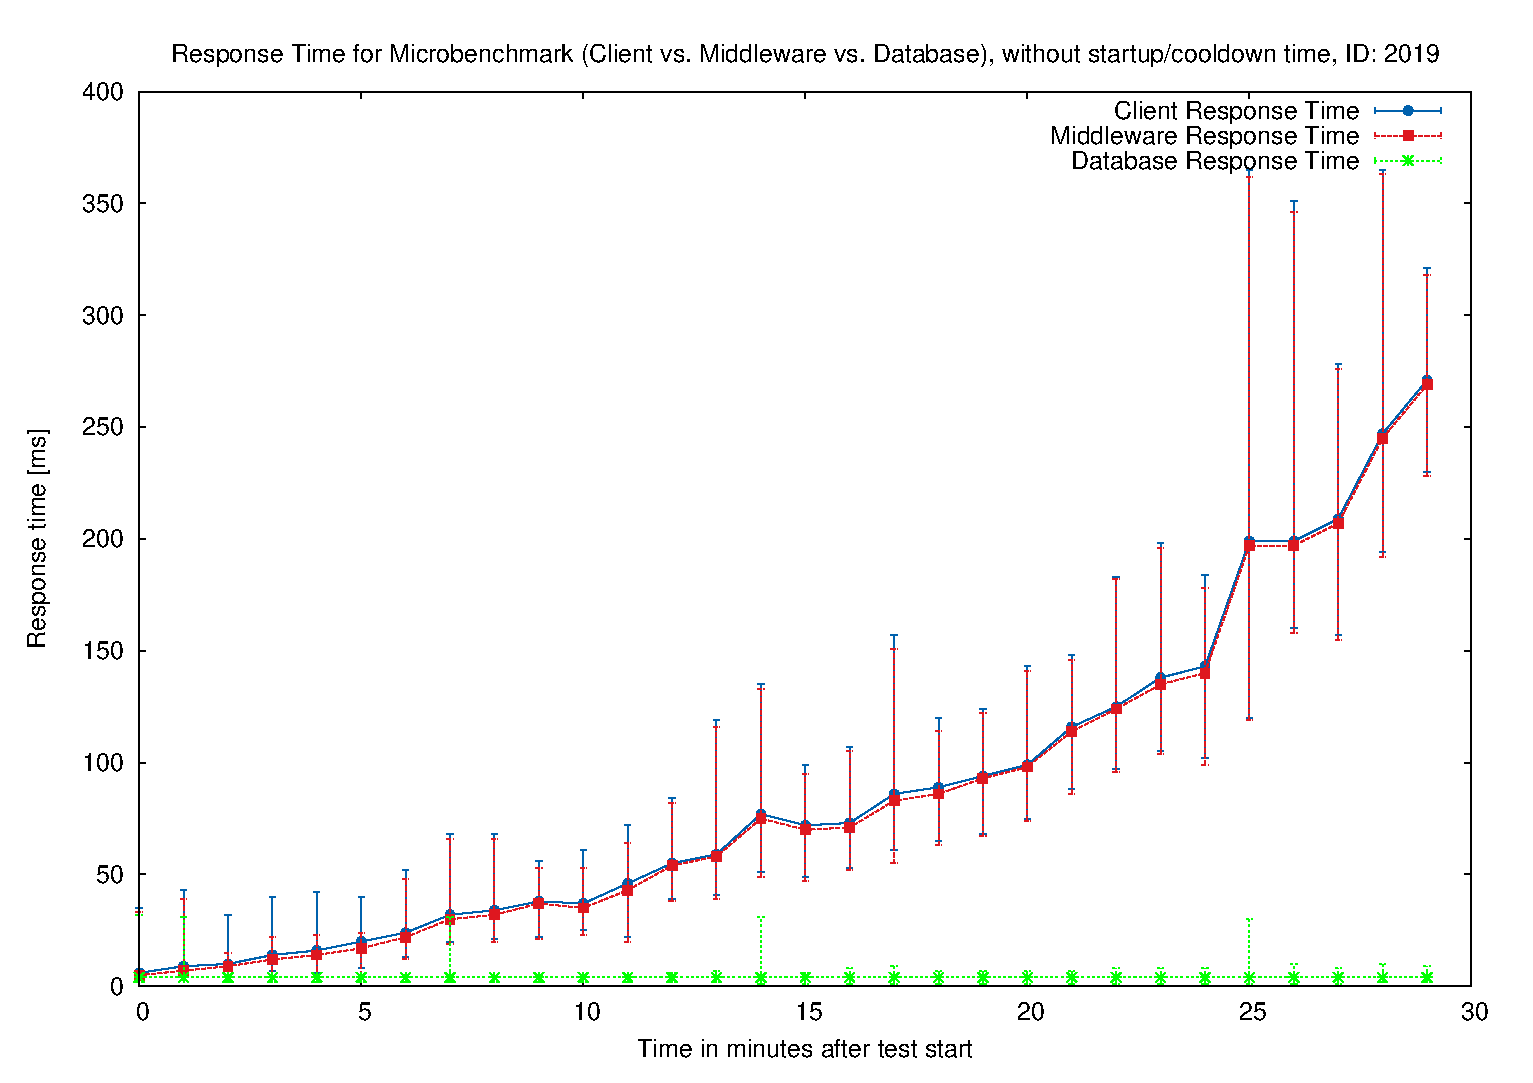
\includegraphics[scale=0.5]{../exported_plots/microbenchmarks/broker_stress_rt.eps}
  \end{center}
  \caption{Response time of Middleware Load Test. The error bars are the 2.5\% and 97.5\% percentiles.}
  \label{fig:BrokerLoadTestResponseTime}
\end{figure}

% ------------------------------
\begin{figure}[H]
        \begin{center}
    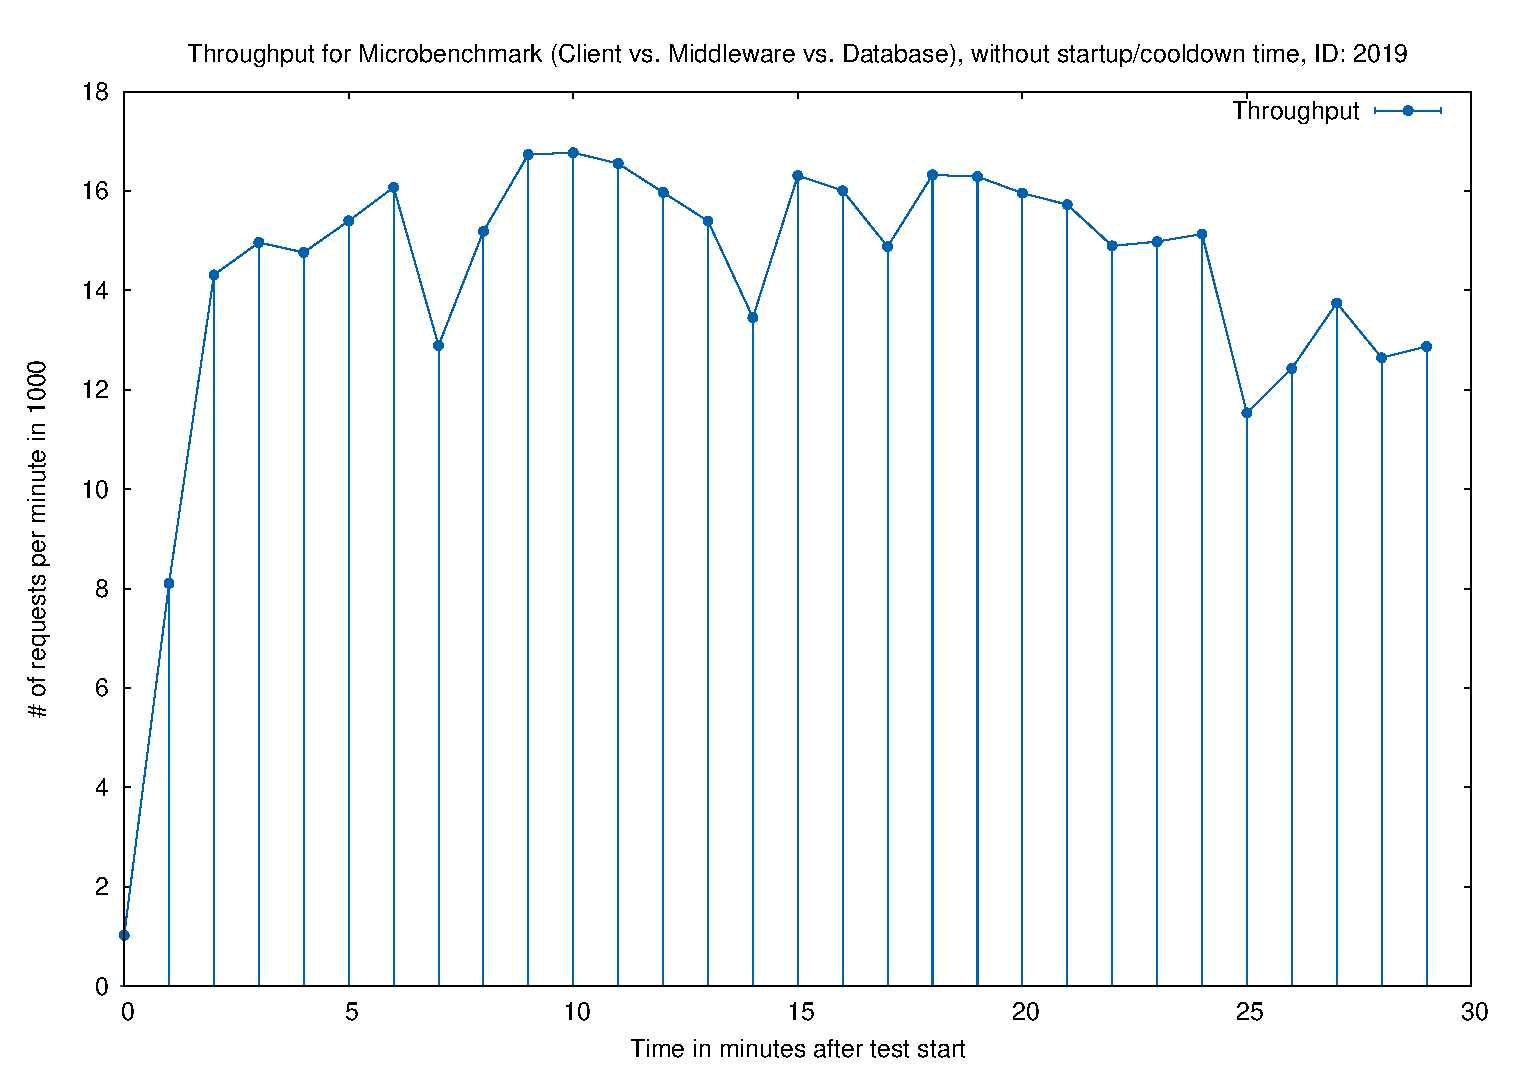
\includegraphics[scale=0.5]{../exported_plots/microbenchmarks/broker_stress_tp.eps}
  \end{center}
  \caption{Througput of Middleware Load Test.}
  \label{fig:BrokerLoadTestThroughput}
\end{figure}



\subsection{Performance Breakup for Different Tiers in the 2h Test}

To find out which components spend how much time, a performance breakup has been conducted for sending and receiving messages.

\subsubsection{Hypothesis}
The 2h test only generates load on the middleware, and load on the database. While the middleware should already be a little stressed out, the database shouldn't have to do too much work. We expect that the system is stable and the database queries are fast.

\begin{figure}[H]
        \begin{center}
    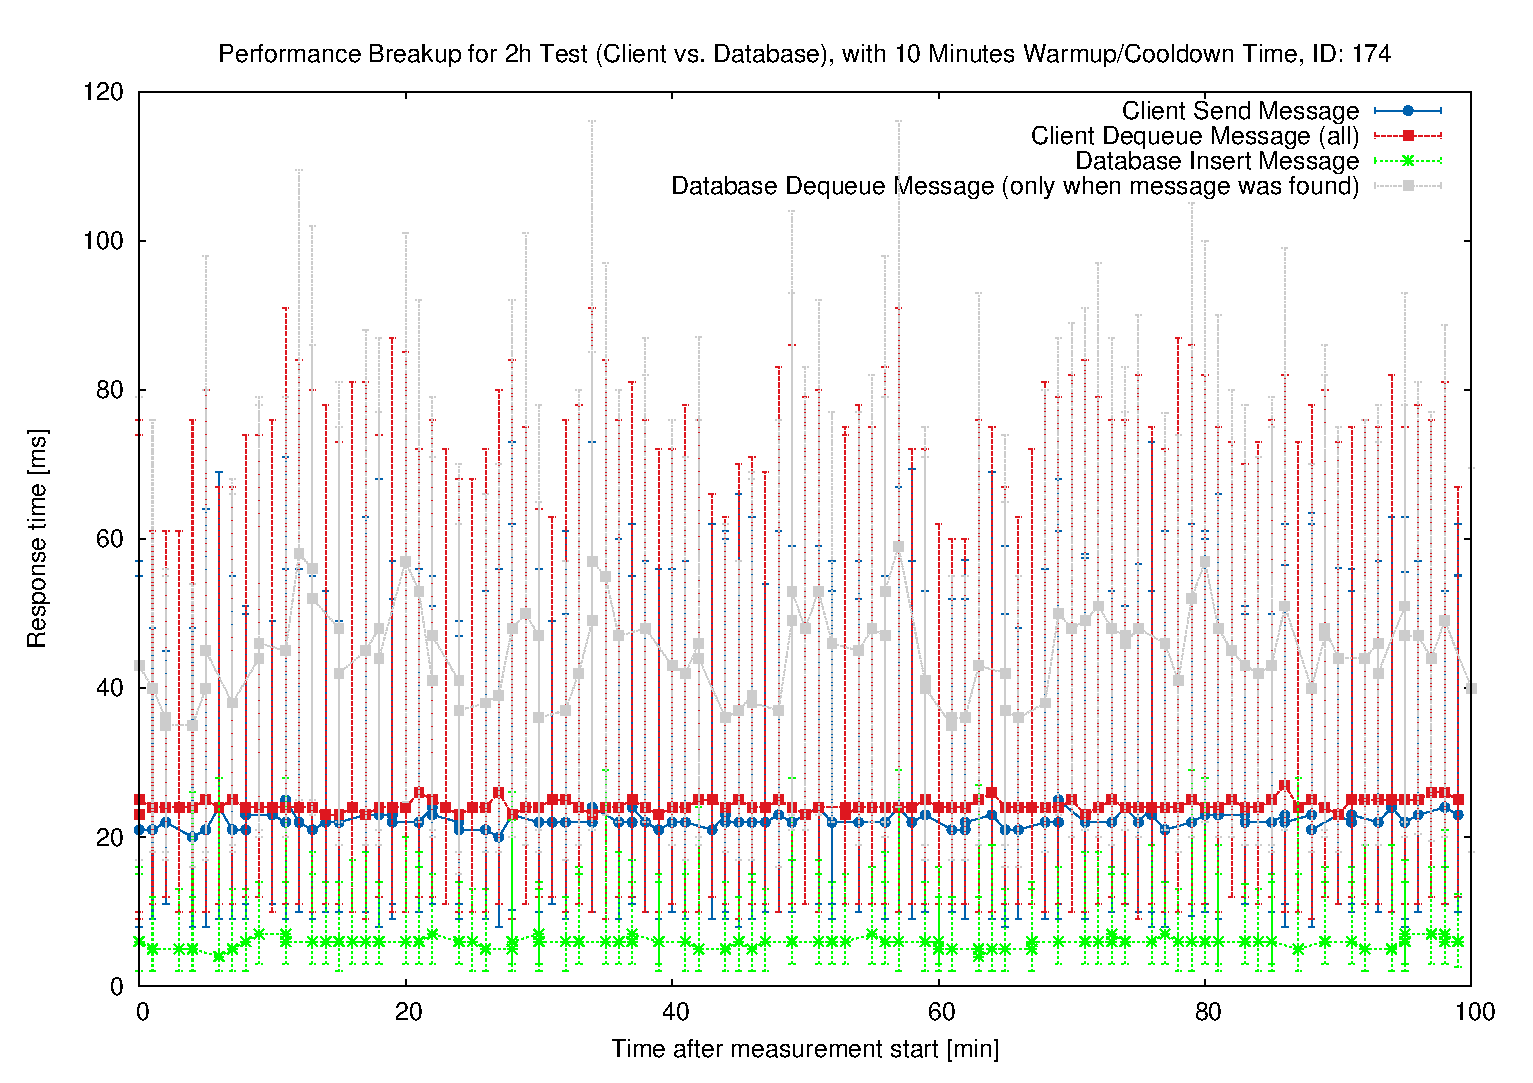
\includegraphics[scale=0.55]{../exported_plots/2h/performance_breakup.eps}
  \end{center}
  \caption{Performance breakup for the 2h test.}
  \label{fig:performancebreakup2h}
\end{figure}

\subsubsection{Interpretation}
As expected, the system runs stable with a median response time between 20ms and 30ms. 95\% of the deque message response time is in between 10ms and 90ms, while the send message response time stays under 60ms-70ms for 97.5\% of the send message requests. Thus while sending messages is a little bit faster (about 2ms-3ms) then dequeing messages, inserting messages is more predictable.


\end{document}
